\begin{name}
	{\tenchude}{Đề thi thử tốt nghiệp THPT năm 2023 - Cụm các trường THPT Huyện Nam Trực}{LỚP TOÁN THẦY PHÁT}{\thoigian}	
\end{name}
\setcounter{ex}{0}\setcounter{bt}{0}
\Opensolutionfile{ans}[ans/ans-2-TT-14-NamTruc-NamDinh-23]
\begin{ex}%[Thi thử tốt nghiệp THPT- Cụm các trường THPT Nam Trực - Nam Định - 23]%[Phạm Tuấn B - EX6]%[2H3Y2-2]
	Trong không gian $Oxyz$, véc-tơ nào sau đây là một véc-tơ pháp tuyến của mặt phẳng $(P)\colon 4x-3y+1=0$?
	\choice
	{\True $\left(4;-3;0\right)$}
	{$\left(4;-3;1\right)$}
	{$\left(4;-3;-1\right)$}
	{$\left(-3;4;0\right)$}
	\loigiai{ Do mặt phẳng $(P)$ có phương trình $4x-3y+1=0$ nên có một véc-tơ pháp tuyến là $\overrightarrow{n}=\left(4;-3;0\right)$.
		}
\end{ex}
\begin{ex}%[Thi thử tốt nghiệp THPT- Cụm các trường THPT Nam Trực - Nam Định - 23]%[Phạm Tuấn B - EX6]%[2D2Y4-1]
	Tập xác định của hàm số $y=\left(x^2-3x-4\right)^{\tfrac{2}{3}}$ là
	\choice
	{$\mathscr{D}=\left(-1;4\right)$}
	{$\mathscr{D}=\mathbb{R}$}
	{$\mathscr{D}=\mathbb{R}\setminus\left\lbrace -1;4\right\rbrace $}
	{\True $\mathscr{D}=\left(-\infty;-1\right)\cup\left(4;+\infty\right)$}
	\loigiai{Do hàm số $y=\left(x^2-3x-4\right)^{\tfrac{2}{3}}$ có $\dfrac{2}{3}\notin\mathbb{Z}$ nên điều kiện xác định là
		$$x^2-3x-4>0\Leftrightarrow\hoac{&x>4\\&x<-1.}$$
		Vậy tập xác định của hàm số là $\mathscr{D}=\left(-\infty;-1\right)\cup\left(4;+\infty\right)$. 
	
}
\end{ex}
\begin{ex}%[Thi thử tốt nghiệp THPT- Cụm các trường THPT Nam Trực - Nam Định - 23]%[Phạm Tuấn B - EX6]%[2D2Y5-1]
	Tập nghiệm của phương trình $\log_2\left(x^2+1\right)=2$ là
	\choice
	{$S=\left\lbrace \sqrt{3}\right\rbrace $}
	{\True $S=\left\lbrace -\sqrt{3};\sqrt{3}\right\rbrace $}
	{$S=\left\lbrace -1;1\right\rbrace $}
	{$S=\left\lbrace 1\right\rbrace $}
	\loigiai{Ta có 
		$$\log_2\left(x^2+1\right)=2\Leftrightarrow x^2+1=4\Leftrightarrow\hoac{&x=\sqrt{3}\\&x=-\sqrt{3}.}$$
		Vậy tập nghiệm của phương trình là $S=\left\lbrace -\sqrt{3};\sqrt{3}\right\rbrace $.
	}
\end{ex}
\begin{ex}%[Thi thử tốt nghiệp THPT- Cụm các trường THPT Nam Trực - Nam Định - 23]%[Phạm Tuấn B - EX6]%[2D3Y3-1]
Gọi $S$ là diện tích của hình phẳng giới hạn bởi các đường $y=3^x$, $y=0$, $x=0$, $x=2$. Mệnh đề nào dưới đây đúng?
\choice
{\True $S=\displaystyle\int\limits_0^23^x\mathrm{\,d}x$}
{$S=\pi\displaystyle\int\limits_0^23^{2x}\mathrm{\,d}x$}
{$S=\pi\displaystyle\int\limits_0^23^x\mathrm{\,d}x$}
{$S=\displaystyle\int\limits_0^23^{2x}\mathrm{\,d}x$}
\loigiai{Diện tích của hình phẳng giới hạn bởi các đường $y=3^x$, $y=0$, $x=0$, $x=2$ là $S=\displaystyle\int\limits_0^23^x\mathrm{\,d}x$.
}
\end{ex}
\begin{ex}%[Thi thử tốt nghiệp THPT- Cụm các trường THPT Nam Trực - Nam Định - 23]%[Phạm Tuấn B - EX6]%[1D3Y4-3]
Cho cấp số nhân $\left(u_n\right)$ có số hạng đầu $u_1=3$ và công bội $q=2$. Số hạng thứ năm của cấp số nhân $\left(u_n\right)$ là
\choice
{$u_5=96$}
{$u_5=32$}
{\True $u_5=48$}
{$u_5=24$}
\loigiai{Do $\left(u_n\right)$ là cấp số nhân có số hạng đầu $u_1=3$ và công bội $q=2$ nên $u_5=u_1\cdot q^4=3\cdot 2^4=48$.
	
}
\end{ex}
\begin{ex}%[Thi thử tốt nghiệp THPT- Cụm các trường THPT Nam Trực - Nam Định - 23]%[Phạm Tuấn B - EX6]%[2D1Y4-1]
Tiệm cận đứng của đồ thị hàm số $y=\dfrac{2x-1}{x-3}$ là đường thẳng có phương trình
\choice
{$x=\dfrac{1}{2}$}
{\True $x=3$}
{$x=-3$}
{$x=2$}
\loigiai{Hàm số $y=\dfrac{2x-1}{x-3}$ có tập xác định $\mathscr{D}=\mathbb{R}\setminus\left\lbrace 3\right\rbrace $.\\
	Suy ra đồ thị hàm số $y=\dfrac{2x-1}{x-3}$ có tiệm cận đứng là đường thẳng $x=3$.
}
\end{ex}
\begin{ex}%[Thi thử tốt nghiệp THPT- Cụm các trường THPT Nam Trực - Nam Định - 23]%[Phạm Tuấn B - EX6]%[2H3Y1-3]
Trong không gian $Oxyz$, cho mặt cầu $(S)$ có phương trình là $\left(x-1\right)^2+\left(y+2\right)^2+\left(z+1\right)^2=4$. Mặt cầu $(S)$ có toạ độ tâm là
\choice
{$\left(-1;2;1\right)$}
{\True $\left(1;-2;-1\right)$}
{$\left(1;-2;1\right)$}
{$\left(1;2;2\right)$}
\loigiai{Do mặt cầu $(S)$ có phương trình là $\left(x-1\right)^2+\left(y+2\right)^2+\left(z+1\right)^2=4$ nên toạ độ tâm là $\left(1;-2;-1\right)$.	
}
\end{ex}
\begin{ex}%[Thi thử tốt nghiệp THPT- Cụm các trường THPT Nam Trực - Nam Định - 23]%[Phạm Tuấn B - EX6]%[2H1Y3-2]
Cho hình chóp $S.ABC$ có đáy $ABC$ là tam giác vuông tại $A$; $AB=3a$, $AC=a$ và đường cao $SA=2a$. Thể tích khối chóp $S.ABC$ bằng
\choice
{$3a^3$}
{\True $a^3$}
{$2a^3$}
{$\dfrac{a^3}{3}$}
\loigiai{Thể tích khối chóp $S.ABC$ là $V=\dfrac{1}{3}\cdot SA\cdot S_{ABC}=\dfrac{1}{3}\cdot 2a\cdot \dfrac{1}{2}\cdot 3a\cdot a=a^3$.
}
\end{ex}
\begin{ex}%[Thi thử tốt nghiệp THPT- Cụm các trường THPT Nam Trực - Nam Định - 23]%[Phạm Tuấn B - EX6]%[1H3Y4-2]
Cho hình chóp $S.ABCD$ có đáy $ABCD$ là hình chữ nhật tâm $I$, cạnh bên $SA$ vuông góc với đáy. Khẳng định nào sau đây đúng?
\choice
{\True $(SCD)\perp(SAD)$}
{$(SBC)\perp(SIA)$}
{$(SCD)\perp(SAI)$}
{$(SBD)\perp(SAC)$}
\loigiai{Do $\heva{&CD\perp AD\\&CD\perp SA}\Rightarrow CD\perp(SAD)\Rightarrow (SCD)\perp(SAD)$.
}
\end{ex}
\begin{ex}%[Thi thử tốt nghiệp THPT- Cụm các trường THPT Nam Trực - Nam Định - 23]%[Phạm Tuấn B - EX6]%[2D1Y5-3]
\immini{Cho hàm số $f(x)=ax^4+bx^2+c\,\big(a,b,c\in\mathbb{R}\big)$ và có bảng biến thiên như hình vẽ bên. Số nghiệm thực dương của phương trình $2f(x)-3=0$ là
\choice
{$1$}
{$4$}
{\True $2$}
{$3$}}
{
\begin{tikzpicture}
	\tkzTabInit[espcl=1.5,lgt=1.5]
	{$x$/0.7,$y'$/0.7,$y$/1.8}
	{$-\infty$,$-1$,$0$,$1$,$+\infty$}
	\tkzTabLine{,-,0,+,0,-,0,+}
	\tkzTabVar{+/$+\infty$,-/$1$,+/$2$,-/$ 1 $,+/$+\infty$}
	\end{tikzpicture}}
\loigiai{Ta có $2f(x)-3=0\Leftrightarrow f(x)=\dfrac{3}{2}$. \\
	Từ bảng biến thiên ta có số nghiệm thực dương của phương trình $2f(x)-3=0$ là $2$.
}
\end{ex}
\begin{ex}%[Thi thử tốt nghiệp THPT- Cụm các trường THPT Nam Trực - Nam Định - 23]%[Phạm Tuấn B - EX6]%[2H2Y1-2]
Cho hình trụ có đường sinh bằng $3r$ và bán kính đáy bằng $r$. Diện tích xung quanh của hình trụ đã cho là
\choice
{$S_{\text{xq}}=8\pi r^2$}
{$S_{\text{xq}}=3\pi r^2$}
{\True $S_{\text{xq}}=6\pi r^2$}
{$S_{\text{xq}}=2\pi r^2$}
\loigiai{Diện tích xung quanh của hình trụ là $S_{\text{xq}}=2\pi r\ell=2\pi\cdot r\cdot 3r=6\pi r^2$.	
}
\end{ex}
\begin{ex}%[Thi thử tốt nghiệp THPT- Cụm các trường THPT Nam Trực - Nam Định - 23]%[Phạm Tuấn B - EX6]%[2D3Y1-1]
Một nguyên hàm của hàm số $f(x)=\dfrac{1}{2x-3}$ là $F(x)$ bằng
\choice
{$-\dfrac{2}{\left(2x-3\right)^2}$}
{$\dfrac{1}{2\left(2x-3\right)^2}$}
{$2\ln\left|2x-3\right|$}
{\True $\dfrac{1}{2}\ln\left|2x-3\right|$}
\loigiai{Do $\displaystyle\int\dfrac{1}{2x-3}\mathrm{\,d}x=\dfrac{1}{2}\ln\left|2x-3\right|+C$  nên $F(x)=\dfrac{1}{2}\ln\left|2x-3\right|$.
}
\end{ex}
\begin{ex}%[Thi thử tốt nghiệp THPT- Cụm các trường THPT Nam Trực - Nam Định - 23]%[Phạm Tuấn B - EX6]%[2D1Y1-1]
Hàm số $y=x^3-3x^2-9x+3$ đồng biến trên khoảng nào dưới đây?
\choice
{$\left(-\infty;+\infty\right)$}
{$\left(-2;+\infty\right)$}
{\True $\left(3;+\infty\right)$}
{$\left(-\infty;1\right)$}
\loigiai{Tập xác định của hàm số là $\mathscr{D}=\mathbb{R}$.\\
	Ta có $y'=3x^2-6x-9$, suy ra $y'=0\Leftrightarrow\hoac{&x=-1\\&x=3.}$\\
	Bảng biến thiên của hàm số như sau
	\begin{center}
		
\begin{tikzpicture}
		\tkzTabInit[espcl=2,lgt=1.5]
		{$x$/0.7,$y'$/0.7,$y$/1.8}
		{$-\infty$,$-1$,$3$,$+\infty$}
		\tkzTabLine{,+,0,-,0,+}
		\tkzTabVar{-/$-\infty$,+/$8$,-/$-24$,+/$+\infty$}
		\end{tikzpicture}
	\end{center}
	Vậy hàm số đồng biến trên khoảng $\left(3;+\infty\right)$.
}
\end{ex}
\begin{ex}%[Thi thử tốt nghiệp THPT- Cụm các trường THPT Nam Trực - Nam Định - 23]%[Phạm Tuấn B - EX6]%[2H3Y1-1]
Trong không gian với hệ trục toạ độ $Oxyz$, cho $\overrightarrow{a}=-\overrightarrow{i}+2\overrightarrow{j}-3\overrightarrow{k}$. Toạ độ của véctơ $\overrightarrow{a}$ là
\choice
{$\left(2;-3;-1\right)$}
{\True $\left(-1;2;-3\right)$}
{$\left(2;-1;-3\right)$}
{$\left(-3;2;-1\right)$}
\loigiai{Do $\overrightarrow{a}=-\overrightarrow{i}+2\overrightarrow{j}-3\overrightarrow{k}$ nên toạ độ của véctơ $\overrightarrow{a}$ là $\left(-1;2;-3\right)$.
	
}
\end{ex}
\begin{ex}%[Thi thử tốt nghiệp THPT- Cụm các trường THPT Nam Trực - Nam Định - 23]%[Phạm Tuấn B - EX6]%[2D1Y5-1]
\immini{Đường cong trong hình bên là đồ thị của một hàm số trong bốn hàm số được liệt kê ở bốn phương án $A$, $B$, $C$, $D$ dưới đây. Hỏi hàm số đó là hàm số nào? 
\choice
{$y=-x^3+3x+1$}
{$y=x^4-x^2+1$}
{\True $y=x^3-3x+1$}
{$y=-x^2+x-1$}}
{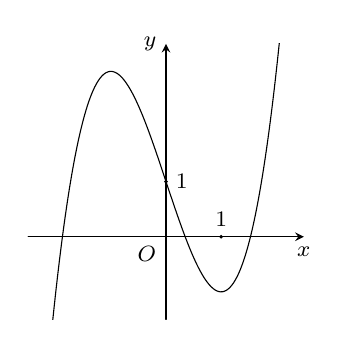
\begin{tikzpicture}[scale=0.7, font=\footnotesize, line join=round, line cap=round, >=stealth]
	\def\xt{-2.5} \def\xp{2.5} \def\yd{-1.5} \def\yt{3.5} 
	\draw[->](\xt,0) -- (0,0)node[below left]{$O$} -- (\xp,0)node[below]{$x$};
	\draw[->](0,\yd)--(0,\yt)node[left]{$y$};
	\begin{scope}
	\clip (\xt,\yd) rectangle (\xp,\yt);
	\draw[smooth,samples=150] plot[domain=\xt:\xp](\x,{1*(\x)^3-3*(\x)+1});
	\end{scope}			
	\foreach \i in {(1,0),(0,1)} \fill \i circle(1pt);
		\path 
	(0,1) node[right]{$1$}
	(1,0) node[above]{$1$};
	\end{tikzpicture}
}
\loigiai{Đồ thị hàm số trên là đồ thị hàm bậc $3$ có $\lim\limits_{x\to +\infty}f(x)=+\infty$.\\
	Suy ra hàm số đó là hàm số $y=x^3-3x+1$.
}
\end{ex}
\begin{ex}%[Thi thử tốt nghiệp THPT- Cụm các trường THPT Nam Trực - Nam Định - 23]%[Phạm Tuấn B - EX6]%[1H3Y3-3]
Cho hình chóp $S.ABC$ có $SA\perp(ABC)$, $SA=a$, $\triangle ABC$ đều cạnh $a$. Tính tang góc giữa đường thẳng $SC$ và mặt phẳng $(SAB)$.
\choice
{\True $\sqrt{\dfrac{3}{5}}$}
{$\sqrt{\dfrac{5}{3}}$}
{$\sqrt{\dfrac{1}{2}}$}
{$\sqrt{2}$}
\loigiai{
	\immini{Trong $\triangle ABC$ hạ $CH\perp AB$. Do $SA\perp(ABC)$ nên $SA\perp CH$ suy ra $CH\perp(SAB)$.\\
		Khi đó $SH$ là hình chiếu của $SC$ xuống mặt phẳng $(SAB)$ suy ra $\widehat{\left(SC,(SAB)\right)}=\widehat{CSH}$.\\
		Mà $\triangle ABC$ đều cạnh $a$ nên $CH=\dfrac{a\sqrt{3}}{2}$.\\
		Xét $\triangle SAC$ vuông tại $A$ có $SC=\sqrt{SA^2+AC^2}=\sqrt{a^2+a^2}=a\sqrt{2}$.\\
		Trong tam giác $SCH$ vuông tại $H$ có $\sin\widehat{CSH}=\dfrac{CH}{SH}=\dfrac{\sqrt{6}}{4}\Rightarrow\tan\widehat{CSH}=\sqrt{\dfrac{3}{5}}$.\\
		Vậy $\tan\widehat{\left(SC,(SAB)\right)}=\sqrt{\dfrac{3}{5}}$.
		}
	{\begin{tikzpicture}[scale=0.8, font=\footnotesize, line join=round, line cap=round, >=stealth]
		\tkzDefPoints{0/0/A, 1.5/-2/B, 4/0/C}
		\coordinate (S) at ($(A)+(0,4)$);
		\coordinate (H) at ($(A)!0.5!(B)$);
		\tkzDrawSegments(S,B S,C S,A B,C A,B S,H)
		\tkzDrawSegments[dashed](A,C C,H)
		\tkzLabelPoints[above](S)
		\tkzLabelPoints[below right](B)
		\tkzLabelPoints[left](A,H)
		\tkzLabelPoints[below right](C)
		\foreach \p in {S,A,B,C,H} \fill (\p) circle(1pt);		
		\end{tikzpicture}}
}
\end{ex}

\begin{ex}%[Thi thử tốt nghiệp THPT- Cụm các trường THPT Nam Trực - Nam Định - 23]%[Phạm Tuấn B - EX6]%[2D1Y1-2]
\immini{Cho hàm số $y=f(x)$ có đồ thị hàm số đạo hàm $y=f'(x)$ như hình vẽ bên. Hàm số $y=f(x)$ đồng biến trên khoảng nào dưới đây?
\choice
{$\left(-1;3\right)$}
{$\left(0;2\right)$}
{$\left(1;+\infty\right)$}
{\True $\left(-1;0\right)$}}
{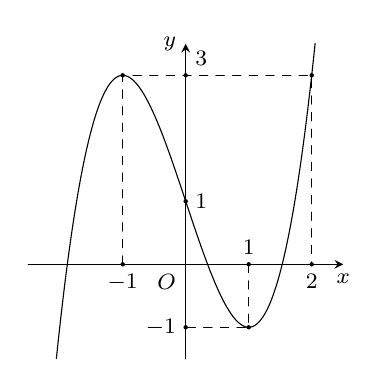
\begin{tikzpicture}[scale=0.8, font=\footnotesize, line join=round, line cap=round, >=stealth]
	\def\xt{-2.5} \def\xp{2.5} \def\yd{-1.5} \def\yt{3.5} 
	\draw[->](\xt,0) -- (0,0)node[below left]{$O$} -- (\xp,0)node[below]{$x$};
	\draw[->](0,\yd)--(0,\yt)node[left]{$y$};
	\begin{scope}
	\clip (\xt,\yd) rectangle (\xp,\yt);
	\draw[smooth,samples=150] plot[domain=\xt:\xp](\x,{1*(\x)^3-3*(\x)+1});
	\end{scope}		
	\draw[dashed](-1,0)--(-1,3)--(2,3)--(2,0) (1,0)--(1,-1)--(0,-1);	
	\foreach \i in {(1,0),(0,1),(-1,0),(-1,3),(0,3),(2,3),(2,0),(0,-1),(1,-1)} \fill \i circle(1pt);
	\path 
	(0,1) node[right]{$1$}
	(0,-1) node[left]{$-1$}
	(0,3) node[above right]{$3$}
	(-1,0) node[below]{$-1$}
	(2,0) node[below]{$2$}
	(1,0) node[above]{$1$};
	\end{tikzpicture}
}
\loigiai{Từ đồ thị hàm số $y=f'(x)$ thì $f'(x)>0,\,\forall x\in\left(-1;0\right)$ nên hàm số đồng biến trên khoảng $\left(-1;0\right)$.
}
\end{ex}
\begin{ex}%[Thi thử tốt nghiệp THPT- Cụm các trường THPT Nam Trực - Nam Định - 23]%[Phạm Tuấn B - EX6]%[2D1Y3-1]
Giá trị nhỏ nhất của hàm số $f(x)=x^4-24x^2-4$ trên $\left[0;19\right]$ bằng
\choice
{$-150$}
{\True $-148$}
{$-149$}
{$-144$}
\loigiai{Hàm số $f(x)=x^4-24x^2-4$ là hàm bậc bốn trùng phương nên liên tục trên $\mathbb{R}$.\\
	Ta có $f'(x)=4x^3-48x$, suy ra $f'(x)=0\Leftrightarrow 4x^3-48x=0\Leftrightarrow\hoac{&x=0\\&x=\sqrt{12}\\&x=-\sqrt{12}\,\left(\text{loại vì}\, -\sqrt{12}\notin\left[0;19\right]\right).}$\\
	Hơn nữa, $f(0)=-4$, $f(19)=121653$, $f\left(\sqrt{12}\right)=-148$ nên $\min\limits_{\left[0;19\right]}f(x)=-148$.
}
\end{ex}
\begin{ex}%[Thi thử tốt nghiệp THPT- Cụm các trường THPT Nam Trực - Nam Định - 23]%[Phạm Tuấn B - EX6]%[2D1Y5-4]
Số giao điểm của đường cong $(C)\colon y=x^3-2x+1$ và đường thẳng $d\colon y=x-1$ là
\choice
{$3$}
{\True $2$}
{$0$}
{$1$}
\loigiai{Xét phương trình hoành độ giao điểm giữa đường cong $(C)$ và đường thẳng $d$ là
	$$x^3-2x+1=x-1\Leftrightarrow x^3-3x+2=0\Leftrightarrow\hoac{&x=1\\&x=-2.}$$
	Vậy số giao điểm là $2$.
}
\end{ex}
\begin{ex}%[Thi thử tốt nghiệp THPT- Cụm các trường THPT Nam Trực - Nam Định - 23]%[Phạm Tuấn B - EX6]%[2D2Y1-2]
Biểu thức $P=\sqrt[3]{x\cdot\sqrt[4]{x}},\,(x>0)$ viết dưới dạng luỹ thừa với số mũ hữu tỷ là
\choice
{\True $P=x^{\tfrac{5}{12}}$}
{$P=x^{\tfrac{1}{12}}$}
{$P=x^{\tfrac{1}{7}}$}
{$P=x^{\tfrac{5}{4}}$}
\loigiai{Ta có $P=\sqrt[3]{x\cdot\sqrt[4]{x}}=\sqrt[3]{x^{1+\tfrac{1}{4}}}=x^{\tfrac{\frac{5}{4}}{3}}=x^{\tfrac{5}{12}}$.
}
\end{ex}
\begin{ex}%[Thi thử tốt nghiệp THPT- Cụm các trường THPT Nam Trực - Nam Định - 23]%[Phạm Tuấn B - EX6]%[2D1Y2-2]
Cho hàm số $y=f(x)$ xác định trên $\mathbb{R}$ và có bảng xét dấu
\begin{center}
	
\begin{tikzpicture}
	\tkzTabInit[espcl=2.5,lgt=1.5]
	{$x$/0.7,$y'$/0.7}
	{$-\infty$,$-3$,$0$,$1$,$2$,$+\infty$}
	\tkzTabLine{,-,0,+,0,+,0,-,0,-}
	%\tkzTabVar{+/$+\infty$,-/$1$,+/$2$,-/$ 1 $,+/$+\infty$}
	\end{tikzpicture}
\end{center}
Hàm số $f(x)$ có bao nhiêu điểm cực trị?
\choice
{$4$}
{$1$}
{$3$}
{\True $2$}
\loigiai{Do $f'(x)$ đổi dấu khi đi qua $x=-3$ và $x=1$ nên hàm $f(x)$ có hai điểm cực trị.
}
\end{ex}
\begin{ex}%[Thi thử tốt nghiệp THPT- Cụm các trường THPT Nam Trực - Nam Định - 23]%[Phạm Tuấn B - EX6]%[2H3Y3-3]
	Trong không gian với hệ toạ độ $Oxyz$, cho mặt cầu có phương trình $\left(x-1\right)^2+\left(y-1\right)^2+\left(z+1\right)^2=36$ cắt trục $Oz$ tại $2$ điểm $A$, $B$. Toạ độ trung điểm của đoạn $AB$ là
	\choice
	{\True $\left(0;0;-1\right)$}
	{$\left(0;0;1\right)$}
	{$\left(1;1;0\right)$}
	{$\left(-1;-1;0\right)$}
	\loigiai{Đường thẳng $Oz$ đi qua điểm $M\left(0;0;-1\right)$ và nhận véctơ $\overrightarrow{k}=\left(0;0;1\right)$ làm một véctơ chỉ phương nên có phương trình là $\heva{&x=0\\&y=0\\&z=-1+t}\,\left(t\in\mathbb{R}\right)$.\\
		Toạ độ hai điểm $A$, $B$ là nghiệm của hệ phương trình
		$$\heva{&x=0\\&y=0\\&z=-1+t\\&\left(x-1\right)^2+\left(y-1\right)^2+\left(z+1\right)^2=36}\Leftrightarrow\heva{&x=0\\&y=0\\&z=-1+t\\&2+t^2=36}\Leftrightarrow\hoac{&\heva{&x=0\\&y=0\\&z=-1+\sqrt{34}}\\&\heva{&x=0\\&y=0\\&z=-1-\sqrt{34}.}}$$
		Vậy trung điểm $I$ của $AB$ có toạ độ là $\left(0;0;-1\right)$.
	}
\end{ex}
\begin{ex}%[Thi thử tốt nghiệp THPT- Cụm các trường THPT Nam Trực - Nam Định - 23]%[Phạm Tuấn B - EX6]%[2D3Y2-1]
	Cho $\displaystyle\int\limits_1^2f(x)\mathrm{\,d}x=3$ và $\displaystyle\int\limits_1^2\left[3f(x)-g(x)\right]\mathrm{\,d}x=10$. Khi đó $\displaystyle\int\limits_1^2g(x)\mathrm{\,d}x$ bằng
	\choice
	{$1$}
	{$-4$}
	{$17$}
	{\True $-1$}
	\loigiai{Ta có $\displaystyle\int\limits_1^2\left[3f(x)-g(x)\right]\mathrm{\,d}x=10\Leftrightarrow \displaystyle\int\limits_1^23f(x)\mathrm{\,d}x-\displaystyle\int\limits_1^2g(x)\mathrm{\,d}x=10\Rightarrow\displaystyle\int\limits_1^2g(x)\mathrm{\,d}x=-1$.
	}
\end{ex}
\begin{ex}%[Thi thử tốt nghiệp THPT- Cụm các trường THPT Nam Trực - Nam Định - 23]%[Phạm Tuấn B - EX6]%[2H1Y3-2]
	Cho lăng trụ đứng $ABC.A'B'C'$ có đáy $ABC$ là tam giác vuông tại $C$, $CA=CB=a$ và $AA'=6a$. Thể tích lăng trụ $ABC.A'B'C'$ bằng
	\choice
	{$2a^3$}
	{\True $3a^3$}
	{$a^3$}
	{$6a^3$}
	\loigiai{
		\immini{Ta có $V_{ABC.A'B'C'}=AA'\cdot S_{ABC}=6a\cdot \dfrac{1}{2}a^2=3a^3$.
		}
		{	\begin{tikzpicture}[line join=round, line cap=round, >=stealth,font=\footnotesize, scale=0.6]
			\tkzDefPoints{0/0/A, 4/0/C, 2.5/-1.5/B, 0/3.5/A'}
			\tkzDefPointBy[translation=from A to A'](B)\tkzGetPoint{B'}
			\tkzDefPointBy[translation=from A to A'](C)\tkzGetPoint{C'}
			\tkzDrawPoints[fill=black,size=3pt](A,B,C,A',B',C')
			\tkzDrawPolygon(A',B',C')
			\tkzDrawSegments(A,A' B,B' C,C' A,B B,C)
			\tkzDrawSegments[dashed](A,C)
			\node[above left]at (A'){$A'$};
			\node[above]at (B'){$B'$};
			\node[above right]at (C'){$C'$};
			\node[below left]at (A){$A$};
			\node[below]at (B){$B$};
			\node[below right]at (C){$C$};
			\end{tikzpicture}
		}
	}
\end{ex}
\begin{ex}%[Thi thử tốt nghiệp THPT- Cụm các trường THPT Nam Trực - Nam Định - 23]%[Phạm Tuấn B - EX6]%[2D2Y5-1]
	Tập nghiệm của phương trình $\log_2\left(x^2+1\right)=2$ là
	\choice
	{$S=\left\{\sqrt{3}\right\}$}
	{\True $S=\left\{-\sqrt{3};\sqrt{3}\right\}$}
	{$S=\left\{-1;1\right\}$}
	{$S=\left\{1\right\}$}
	\loigiai{Ta có $\log_2\left(x^2+1\right)=2\Leftrightarrow x^2+1=4\Leftrightarrow\hoac{&x=\sqrt{3}\\&x=-\sqrt{3}.}$\\
		Vậy tập nghiệm của phương trình là $S=\left\{-\sqrt{3};\sqrt{3}\right\}$.
	}
\end{ex}
\begin{ex}%[Thi thử tốt nghiệp THPT- Cụm các trường THPT Nam Trực - Nam Định - 23]%[Phạm Tuấn B - EX6]%[2D2Y6-1]
	Tập nghiệm của bất phương trình $\left(\dfrac{2}{3}\right)^{4x}\leq\left(\dfrac{3}{2}\right)^{2-x}$ là
	\choice
	{$\left[\dfrac{2}{5};+\infty\right)$}
	{$\left(-\infty;-\dfrac{2}{3}\right]$}
	{\True $\left[-\dfrac{2}{3};+\infty\right)$}
	{$\left(-\infty;\dfrac{2}{5}\right]$}
	\loigiai{
		Ta có 
		$$\left(\dfrac{2}{3}\right)^{4x}\leq\left(\dfrac{3}{2}\right)^{2-x}\Leftrightarrow\left(\dfrac{3}{2}\right)^{-4x}\leq\left(\dfrac{3}{2}\right)^{2-x}\Leftrightarrow -4x\leq 2-x\Leftrightarrow x\geq-\dfrac{2}{3}.$$
		Vậy tập nghiệm của bất phương trình là $\left[-\dfrac{2}{3};+\infty\right)$.
	}
\end{ex}
\begin{ex}%[Thi thử tốt nghiệp THPT- Cụm các trường THPT Nam Trực - Nam Định - 23]%[Phạm Tuấn B - EX6]%[2D1Y1-1]
	Trong các hàm số sau, hàm số nào đồng biến trên $\mathbb{R}$?
	\choice
	{$f(x)=x^3-4x+1$}
	{$f(x)=\dfrac{2x-1}{x+1}$}
	{\True $f(x)=x^3-3x^2+3x+4$}
	{$f(x)=x^4-2x^2-4$}
	\loigiai{Hàm số $y=\dfrac{2x-1}{x+1}$ có tập xác định $\mathscr{D}=\mathbb{R}\setminus\left\{-1\right\}$ nên không đồng biến trên $\mathbb{R}$.\\
		Hàm số $y=x^4-2x^2-4$ luôn có cực trị nên không đồng biến trên $\mathbb{R}$.\\
		Hàm số $y=x^3-4x+1$ có $y'=3x^2-4$ nên $y'=0$ có hai nghiệm phân biệt. Suy ra hàm số $y=x^3-4x+1$ không đồng biến trên $\mathbb{R}$.\\
		Hàm số $y=x^3-3x^2+3x+4$ có $y'=3x^2-6x+3=3\left(x-1\right)^2\ge 0,\,\forall x\in\mathbb{R}$ nên hàm số luôn đồng biến trên $\mathbb{R}$.
	}
\end{ex}
\begin{ex}%[Thi thử tốt nghiệp THPT- Cụm các trường THPT Nam Trực - Nam Định - 23]%[Phạm Tuấn B - EX6]%[2H2B1-2]
	Cho tam giác $ABC$ vuông cân tại $A$, có cạnh $AB=a$. Gọi $H$ là trung điểm của $BC$. Thể tích của khối nón tạo thành khi quay hình tam giác $ABC$ xung quanh trục $AH$ là
	\choice
	{$\dfrac{\sqrt{3}\pi a^3}{12}$}
	{\True $\dfrac{\sqrt{2}\pi a^3}{12}$}
	{$\dfrac{\sqrt{2}\pi a^3}{6}$}
	{$\dfrac{\pi a^3}{12}$}
	\loigiai{\immini{Do tam giác $ABC$ vuông cân tại $A$ nên $AH\perp BC$ và $AH=HB=HC=\dfrac{a\sqrt{2}}{2}$.\\
			Suy ra khi quay hình tam giác $ABC$ xung quanh trục $AH$ sẽ tạo ra khối nón có chiều cao là $AH$ và bán kính đáy $r=HB$.\\
			Vậy thể tích khối nón là $V=\dfrac{1}{3}\cdot AH\cdot \pi HB^2=\dfrac{1}{3}\cdot\pi\cdot\left(\dfrac{a\sqrt{2}}{2}\right)^3=\dfrac{a^3\pi\sqrt{2}}{12}$.
		}
		{\begin{tikzpicture}[scale=0.7, font=\footnotesize, line join=round, line cap=round, >=stealth]
			\draw[dashed] (0:0) arc(180:0:{3} and {.9});
			\draw (0:0) arc(180:360:{3} and {.9});
			\coordinate (A) at (3,4.5);
			\coordinate (H) at (3,0);
			\coordinate (B) at (0,0);
			\coordinate (C) at (6,0);
			\path (B) arc (180:-75:{3} and {.8})coordinate (M);
			\path (B) arc (180:40:{3} and {.8})coordinate (N);
			\draw (B)--(A)--(C);
			\draw[dashed] (A)--(H)--(B)(H)--(C);
			\foreach \d/\g in{A/90,H/130,B/180,C/0}
			\draw[fill=black](\d)circle(1pt)node[shift={(\g:0.35)}]{$\d$};
			\end{tikzpicture}
		}
	}
\end{ex}
\begin{ex}%[Thi thử tốt nghiệp THPT- Cụm các trường THPT Nam Trực - Nam Định - 23]%[Phạm Tuấn B - EX6]%[2D3B1-1]
Tìm nguyên hàm của hàm số $f(x)=\mathrm{e}^x\left(1-\dfrac{2\mathrm{e}^{-x}}{x^5}\right)$.
\choice
{\True $\displaystyle\int f(x)\mathrm{\,d}x=\mathrm{e}^x+\dfrac{1}{2x^4}+C$}
{$\displaystyle\int f(x)\mathrm{\,d}x=\mathrm{e}^x-\dfrac{1}{2x^4}+C$}
{$\displaystyle\int f(x)\mathrm{\,d}x=\mathrm{e}^x-\dfrac{2}{x^4}+C$}
{$\displaystyle\int f(x)\mathrm{\,d}x=\mathrm{e}^x+\dfrac{2}{x^4}+C$}
\loigiai{Ta có 
	\allowdisplaybreaks
	\begin{eqnarray*}
	\displaystyle\int f(x)\mathrm{\,d}x&=&\displaystyle\int \mathrm{e}^x\left(1-\dfrac{2\mathrm{e}^{-x}}{x^5}\right)\mathrm{\,d}x=	\displaystyle\int \left(\mathrm{e}^x-\dfrac{2}{x^5}\right)\mathrm{\,d}x=\mathrm{e}^x+\dfrac{1}{2x^4}+C.
	\end{eqnarray*}	
}
\end{ex}
\begin{ex}%[Thi thử tốt nghiệp THPT- Cụm các trường THPT Nam Trực - Nam Định - 23]%[Phạm Tuấn B - EX6]%[2H3B2-4]
Trong không gian với hệ toạ độ $Oxyz$, phương trình mặt phẳng $(P)$ cắt ba trục toạ độ lần lượt tại $A$, $B$, $C$ sao cho $M\left(1;2;3\right)$ là trọng tâm tam giác $ABC$ là
\choice
{\True $6x+3y+2z-18=0$}
{$x+2y+3z=0$}
{$6x-3y+2z-18=0$}
{$\hoac{&6x+3y+2z-18=0\\&x+2y+3z=0}$}
\loigiai{
	Gọi toạ độ của ba điểm $A$, $B$, $C$ lần lượt là $\left(a;0;0\right)$, $\left(0;b;0\right)$ và $\left(0;0;c\right)$. \\
	Do $M\left(1;2;3\right)$ là trọng tâm của tam giác $ABC$ nên
	$$\heva{&\dfrac{a+0+0}{3}=1\\&\dfrac{0+b+0}{3}=2\\&\dfrac{0+0+c}{3}=3}\Leftrightarrow\heva{&a=3\\&b=6\\&c=9.}$$
	Khi đó phương trình mặt phẳng $(P)$ là
	$$\dfrac{x}{3}+\dfrac{y}{6}+\dfrac{z}{9}=1\Leftrightarrow 6x+3y+2z-18=0.$$
}
\end{ex}
\begin{ex}%[Thi thử tốt nghiệp THPT- Cụm các trường THPT Nam Trực - Nam Định - 23]%[Phạm Tuấn B - EX6]%[2H1B3-3]
Cho khối chóp $S.ABCD$ có đáy là hình bình hành tâm $O$, biết thể tích khối chóp $S.OAD$ bằng $10$cm$^3$. Thể tích khối chóp $S.ABCD$ bằng
\choice
{$20$cm$^3$}
{$30$cm$^3$}
{$25$cm$^3$}
{\True $40$cm$^3$}
\loigiai{Do $S_{ABCD}=4S_{OAD}\Rightarrow V_{S.ABCD}=4\cdot V_{S.OAD}=40$cm$^3$.
}
\end{ex}

\begin{ex}%[Thi thử tốt nghiệp THPT- Cụm các trường THPT Nam Trực - Nam Định - 23]%[Phạm Tuấn B - EX6]%[2D1B4-2]
Số các giá trị nguyên của tham số $m$ thuộc $\left[-2023;2023\right]$ để đồ thị hàm số $y=\dfrac{2x+4}{x-m}$ có tiệm cận đứng nằm bên trái trục tung là
\choice
{$4046$}
{$4044$}
{\True $2022$}
{$2023$}
\loigiai{Đề đồ thị hàm số $y=\dfrac{2x+4}{x-m}$ có tiệm cận đứng nằm bên trái trục tung thì
	$$\heva{&2m+4\neq 0\\&m<0}\Leftrightarrow\heva{&m\neq -2\\&m<0.}$$
	Do $m$ nguyên và thuộc $\left[-2023;2023\right]$ suy ra có $2022$ giá trị nguyên của tham số $m$ thoả mãn yêu cầu đề bài.
}
\end{ex}

\begin{ex}%[Thi thử tốt nghiệp THPT- Cụm các trường THPT Nam Trực - Nam Định - 23]%[Phạm Tuấn B - EX6]%[2H2B2-2]
Cho hình chóp tam giác đều $S.ABC$ có cạnh đáy bằng $a$ và cạnh bên bằng $a\sqrt{2}$. Bán kính mặt cầu ngoại tiếp hình chóp $S.ABC$ là
\choice
{$\dfrac{a\sqrt{6}}{4}$}
{$\dfrac{3a}{5}$}
{$\dfrac{a\sqrt{3}}{5}$}
{\True $\dfrac{a\sqrt{15}}{5}$}
\loigiai{\immini{Gọi $G$ là tâm đường tròn ngoại tiếp tam giác đều $ABC$ cạnh $a$.\\
		Suy ra $AG=\dfrac{a\sqrt{3}}{3}$ và $SG\perp(ABC)$.\\
	    Trên $SG$ lấy điểm $I$ sao cho $IS=IA$.\\
		Do $SG\perp(ABC)$ nên $IA=IB=IC$.\\
		Suy ra $I$ là tâm mặt cầu ngoại tiếp hình chóp $S.ABC$.\\
		Qua $I$ kẻ đường thẳng $d$ vuông góc với $SA$ cắt $SA$ tại $N$.\\
		Do $IS=IA$ nên $N$ là trung điểm $SA\Rightarrow SN=\dfrac{SA}{2}$.\\
	    Xét hai tam giác $SNI$ và $SGA$ có $\heva{&\widehat{S}\,\text{chung}\\&\widehat{SNI}=\widehat{SGA}=90^\circ.}$\\
	    Do đó $\triangle SNI \sim\triangle SGA$ suy ra 
	    $$\dfrac{SN}{SG}=\dfrac{SI}{SA}\Leftrightarrow SI=\dfrac{SA\cdot SN}{SG}=\dfrac{SA^2}{2SG}.$$
	    Xét $\triangle SGA$ vuông tại $G$ có $$SG=\sqrt{SA^2-AG^2}=\sqrt{2a^2-\dfrac{a^2}{3}}=\dfrac{a\sqrt{15}}{3}.$$
		Vậy $R=IS=\dfrac{2a^2}{2\cdot\dfrac{a\sqrt{15}}{3}}=\dfrac{a\sqrt{15}}{5}$.
	}
	{\begin{tikzpicture}[scale=.6, line join = round, line cap = round]
		\tikzset{label style/.style={font=\footnotesize}}
		\tkzDefPoints{0/0/A,9/0/C,3/-3/B}
		\coordinate (N) at ($(A)!0.5!(S)$);
		\coordinate (M) at ($(C)!0.5!(B)$);
		\tkzCentroid(A,B,C)    \tkzGetPoint{G}
		\coordinate (S) at ($(G)+(0,6)$);
		\coordinate (I) at ($(G)+(0,2)$);
		\coordinate (d) at ($(I)!1.3!(N)$);
		\tkzDrawPolygon(S,A,B,C)
		\tkzDrawSegments(S,B d,N)
		\tkzDrawSegments[dashed](A,C N,I G,S A,M A,I)
		\tkzDrawPoints[fill=black](A,B,C,S,G,N,I,M)
		\tkzLabelPoints[above](S,d)
		\tkzLabelPoints[below](B,G)
		\tkzLabelPoints[left](A)
		\tkzLabelPoints[left](N)
		\tkzLabelPoints[right](C,I)
		\begin{scope}[on background layer]\path[white]node{MDD-139};\end{scope}
		\end{tikzpicture}
	}
}
\end{ex}
\begin{ex}%[Thi thử tốt nghiệp THPT- Cụm các trường THPT Nam Trực - Nam Định - 23]%[Phạm Tuấn B - EX6]%[2D3B3-1]
Gọi diện tích hình phẳng giới hạn bởi đồ thị hàm số $(C)\colon y=\dfrac{-3x-1}{x-1}$ và hai trục toạ độ là $S$. Tính $S$?
\choice
{\True $S=4\ln\dfrac{4}{3}-1$}
{$S=\ln\dfrac{4}{3}-1$}
{$S=1-\ln\dfrac{4}{3}$}
{$S=4\ln\dfrac{4}{3}$}
\loigiai{Phương trình hoành độ giao điểm của đồ thị $(C)$ với trục hoành là
	$$\dfrac{-3x-1}{x-1}=0\Leftrightarrow x=-\dfrac{1}{3}.$$
	Khi đó diện tích hình phẳng giới hạn bởi đồ thị hàm số $(C)\colon y=\dfrac{-3x-1}{x-1}$ và hai trục toạ độ là
	$$S=\displaystyle\int\limits_{-\tfrac{1}{3}}^0\left|\dfrac{-3x-1}{x-1}\right|\mathrm{\,d}x=\left|\displaystyle\int\limits_{-\tfrac{1}{3}}^0\dfrac{-3x-1}{x-1}\mathrm{\,d}x\right|=\left|\displaystyle\int\limits_{-\tfrac{1}{3}}^0\left(-3-\dfrac{4}{x-1}\right)\mathrm{\,d}x\right|=\left|-3x-4\ln\left|x-1\right|\Big|_{-\tfrac{1}{3}}^0\right|=4\ln\dfrac{4}{3}-1.$$
}
\end{ex}

\begin{ex}%[Thi thử tốt nghiệp THPT- Cụm các trường THPT Nam Trực - Nam Định - 23]%[Phạm Tuấn B - EX6]%[1D2B5-2]
	Một hộp chứa $11$ quả cầu gồm $5$ quả cầu màu xanh và $6$ quả cầu màu đỏ. Lấy ngẫu nhiên đồng thời $2$ quả cầu từ hộp đó. Tính xác suất để lấy được $2$ quả khác màu.
	\choice
	{$\dfrac{8}{11}$}
	{$\dfrac{5}{11}$}
	{\True $\dfrac{6}{11}$}
	{$\dfrac{5}{22}$}
	\loigiai{Số phần tử của không gian mẫu là $\mathrm{n}\left(\Omega\right)=\mathrm{C}_{11}^2$.\\
		Gọi $A$ là biến có lấy được $2$ quả khác màu. Suy ra $\mathrm{n}(A)=\mathrm{C}_5^1\cdot\mathrm{C}_6^1=30$.\\
		Vậy xác suất để lấy được $2$ quả khác màu là $\mathrm{P}(A)=\dfrac{30}{\mathrm{C}_{11}^2}=\dfrac{6}{11}$.
	}
\end{ex}
\begin{ex}%[Thi thử tốt nghiệp THPT- Cụm các trường THPT Nam Trực - Nam Định - 23]%[Phạm Tuấn B - EX6]%[2D1B5-3]
	Tìm tất cả các giá trị thực của tham số $m$ để phương trình $\left|x^4-2x^2-3\right|=2m-1$ có đúng $6$ nghiệm thực phân biệt.
	\choice
	{$3<m<4$}
	{\True $2<m<\dfrac{5}{2}$}
	{$1<m<\dfrac{3}{2}$}
	{$4<m<5$}
	\loigiai{
		\immini{
		Xét hàm số $f(x)=x^4-2x^2-3$ có tập xác định $\mathscr{D}=\mathbb{R}$.\\
		Ta có $f'(x)=4x^4-4x$ nên $f'(x)=0\Leftrightarrow\hoac{&x=0\\&x=\pm 1.}$\\
		Khi đó ta có đồ thị của hàm $y=x^4-4x^2-3$ như hình vẽ bên.
	}
{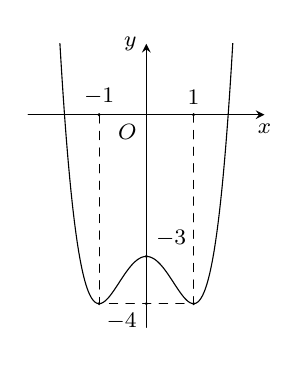
\begin{tikzpicture}[scale=0.6, font=\footnotesize, line join=round, line cap=round, >=stealth]
	\def\xt{-2.5} \def\xp{2.5} \def\yd{-4.5} \def\yt{1.5} 
	\draw[->](\xt,0) -- (0,0)node[below left]{$O$} -- (\xp,0)node[below]{$x$};
	\draw[->](0,\yd)--(0,\yt)node[left]{$y$};
	\begin{scope}
	\clip (\xt,\yd) rectangle (\xp,\yt);
	\draw[smooth,samples=150] plot[domain=\xt:\xp](\x,{1*(\x)^4-2*(\x)^2-3});
	\end{scope}		
	\draw[dashed](-1,0)--(-1,-4)--(1,-4)--(1,0);	
	\foreach \i in {(1,0),(0,-3),(-1,0),(-1,-4),(1,-4),(0,-4)} \fill \i circle(1pt);
	\path 
	(0,-3) node[above right]{$-3$}
	(0,-4) node[below left]{$-4$}
	(-1,0) node[above]{$-1$}
	(1,0) node[above]{$1$};
	\end{tikzpicture}
}
\immini{Từ đồ thị hàm số $y=x^4-2x^2-3$ ta có đồ thị của hàm số $y=\left|x^4-2x^2-3\right|$ như hình vẽ bên.\\
	Từ đồ thị của hàm số $y=\left|x^4-2x^2-3\right|$ suy ra để phương trình 
	$$\left|x^4-2x^2-3\right|=2m-1$$
	có đúng $6$ nghiệm thực phân biệt thì $3<2m-1<4\Leftrightarrow2<m<\dfrac{5}{2}$.
}
{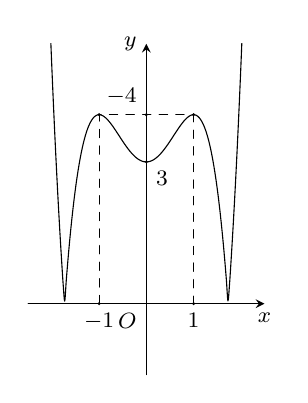
\begin{tikzpicture}[scale=0.6, font=\footnotesize, line join=round, line cap=round, >=stealth]
	\def\xt{-2.5} \def\xp{2.5} \def\yd{-1.5} \def\yt{5.5} 
	\draw[->](\xt,0) -- (0,0)node[below left]{$O$} -- (\xp,0)node[below]{$x$};
	\draw[->](0,\yd)--(0,\yt)node[left]{$y$};
	\begin{scope}
	\clip (\xt,\yd) rectangle (\xp,\yt);
	\draw[smooth,samples=150] plot[domain=\xt:\xp](\x,{abs(1*(\x)^4-2*(\x)^2-3)});
	\end{scope}		
	\draw[dashed](-1,0)--(-1,4)--(1,4)--(1,0);	
	\foreach \i in {(1,0),(0,3),(-1,0),(-1,4),(1,4),(0,4)} \fill \i circle(1pt);
	\path 
(0,3) node[below right]{$3$}
(0,4) node[above left]{$-4$}
(-1,0) node[below]{$-1$}
(1,0) node[below]{$1$};
	\end{tikzpicture}
}
	}
\end{ex}
\begin{ex}%[Thi thử tốt nghiệp THPT- Cụm các trường THPT Nam Trực - Nam Định - 23]%[Phạm Tuấn B - EX6]%[2H2B2-6]
	Cho lập phương $ABCD.A'B'C'D'$ có cạnh bằng $a$. Gọi $V_1$, $V_2$, $V_3$ lần lượt là thể tích của khối trụ ngoại tiếp, khối cầu nội tiếp, khối cầu ngoại tiếp hình lập phương $ABCD.A'B'C'D'$. Tính giá trị $P=\dfrac{V_1+V_2}{V_3}$.
	\choice
	{$P=\dfrac{\sqrt{3}}{3}$}
	{$P=\dfrac{4\sqrt{3}}{3}$}
	{$P=\dfrac{2\sqrt{3}}{3}$}
	{\True $P=\dfrac{4\sqrt{3}}{9}$}
	\loigiai{\immini{Do $ABCD.A'B'C'D'$ là hình lập phương có cạnh bằng $a$ nên bán kính đường tròn ngoại tiếp hình vuông $ABCD$ là $R_1=\dfrac{a\sqrt{2}}{2}$; bán kính khối cầu nội tiếp hình lập phương là $R_2=\dfrac{a}{2}$ và bán kính khối cầu ngoại tiếp hình lập phương là $R_3=\dfrac{a\sqrt{3}}{2}$.\\
			\begin{itemize}
				\item Thể tích khối trụ ngoại tiếp hình lập phương là $V_1=AA'\cdot\pi R_1^2=\dfrac{\pi a^3}{2}$.
				\item Thể tích khối cầu nội tiếp hình lập phương là $V_2=\dfrac{4}{3}\pi R_2^3=\dfrac{\pi a^3}{6}$.
				\item Thể tích khối cầu ngoại tiếp hình lập phương là $V_3=\dfrac{4}{3}\pi R_3^3=\dfrac{\pi a^3\sqrt{3}}{2}$.
			\end{itemize}
		Vậy $P=\dfrac{V_1+V_2}{V_3}=\dfrac{\tfrac{1}{2}+\tfrac{1}{6}}{\tfrac{\sqrt{3}}{2}}=\dfrac{4\sqrt{3}}{9}$.
		}
		{\begin{tikzpicture}[scale=0.8,font=\footnotesize,line join = round, line cap = round, >= stealth]
			\tkzDefPoints{0/0/A, 3/0/x, 1.2/1.8/y, 0/3/z}
			\coordinate (B) at ($(A)+(y)$);
			\coordinate (C) at ($(B)+(x)$);
			\coordinate (D) at ($(A)+(x)$);
			
			\coordinate (A') at ($(A)+(z)$);
			\coordinate (B') at ($(B)+(z)$);
			\coordinate (C') at ($(C)+(z)$);
			\coordinate (D') at ($(D)+(z)$);
			
			\coordinate (O) at ($(A)!0.5!(C)$);
			
			\tkzDrawPolygon(A',B',C',D')
			\tkzDrawSegments[](C,C' A,D D,D' D,C A,A')
			\tkzDrawSegments[dashed](B,D A,C A,B B,C B,B')
			\tkzDrawPoints[fill=black](A,B,C,D,A',B',C',D',O)
			\tkzLabelPoints[left](B)
			\tkzLabelPoints[right](C,D)
			\tkzLabelPoints[above](B',C',A',D')
			\tkzLabelPoints[below](O,A)
			\end{tikzpicture}
		}
	}
\end{ex}
\begin{ex}%[Thi thử tốt nghiệp THPT- Cụm các trường THPT Nam Trực - Nam Định - 23]%[Phạm Tuấn B - EX6]%[2D2B4-7]
	\immini{
		Cho $a$, $b$ là các số thực dương khác $1$, đường thẳng $(d)$ song song với
		trục hoành cắt trục tung, đồ thị hàm số $y=a^x$, đồ thị hàm số $y=b^x$ lần lượt tại $H$, $M$, $N$ (như hình bên). Biết $HM=3MN$, mệnh đề nào sau đây đúng?
		\choice
		{$4a=3b$}
		{\True $b^4=a^3$}
		{$b^3=a^4$}
		{$3a=4b$}}
	{
		\begin{tikzpicture}[scale=0.7,>=stealth, font=\footnotesize, line join=round, line cap=round]
		\def\xmin{-2} \def\xmax{4} \def\ymax{5}
		\draw[->] (\xmin,0)--(\xmax,0) node [below]{$x$};
		\draw[->] (0,-0.9)--(0,\ymax) node [left]{$y$};
		\draw[fill=black] (0,0)node[below left]{$O$} circle (1pt);
		\clip (-2,-1) rectangle (5,5.2);
		\draw[smooth,samples=300,domain=-2:2.3] plot(\x,{2^(\x)})node[right]{$y=b^x$};
		\draw[smooth,samples=300,domain=-2:1.7] plot(\x,{(2.52)^(\x)})node[left]{$y=a^x$};
		\draw (-1,4)--(5,4);
		\draw[fill=black] (2,4)node[above right]{$N$} circle(1pt);
		\draw[fill=black] (1.5,4)node[above left]{$M$} circle(1pt);
		\draw[fill=black] (0,4)node[above right]{$H$} circle(1pt);
		\draw[dashed] (1.5,4)--(1.5,0);
		\draw[dashed](2,4)--(2,0);
		\draw[fill=black] (1.5,0)node[below]{$x_M$} circle(1pt);
		\draw[fill=black] (2,0)node[below right]{$x_N$} circle(1pt);
		\begin{scope}[on background layer]\path[white]node{MDD-327};\end{scope}
		\end{tikzpicture}}
	\loigiai{
		Do $HM=3MN\Rightarrow x_M=\dfrac{3}{4}x_N$.\\
		Hơn nữa do $y_M=y_N$ nên $a^{\tfrac{3}{4}x_N}=b^{x_N}\Leftrightarrow a^3=b^4$.
	}
\end{ex}
\begin{ex}%[Thi thử tốt nghiệp THPT- Cụm các trường THPT Nam Trực - Nam Định - 23]%[Phạm Tuấn B - EX6]%[2D3B2-1]
	Biết $\displaystyle\int\limits_0^1\dfrac{2x^2+3x+3}{x^2+2x+1}\mathrm{\,d}x=a-\ln b$ với $a$, $b$ là các số nguyên dương. Tính $P=a^2+b^2$.
	\choice
	{\True $13$}
	{$5$}
	{$4$}
	{$10$}
	\loigiai{Ta có
		\allowdisplaybreaks
		\begin{eqnarray*}
			&&\displaystyle\int\limits_0^1\dfrac{2x^2+3x+3}{x^2+2x+1}\mathrm{\,d}x=\displaystyle\int\limits_0^1\dfrac{2x^2+4x+2-x-1+2}{x^2+2x+1}\mathrm{\,d}x=\displaystyle\int\limits_0^1\left(2+\dfrac{2}{\left(x+1\right)^2}-\dfrac{1}{x+1}\right)\mathrm{\,d}x\\
			&=&\left(2x-\ln\left|x+1\right|-\dfrac{2}{x+1}\right)\Big|_0^1=\left(2-\ln 2-1\right)-\left(-2\right)=3-\ln 2.
		\end{eqnarray*}
		Vậy $a=3$ và $b=2$ nên $P=13$.
	}
\end{ex}
\begin{ex}%[Thi thử tốt nghiệp THPT- Cụm các trường THPT Nam Trực - Nam Định - 23]%[Phạm Tuấn B - EX6]%[2D2K6-5]
	Có bao nhiêu giá trị nguyên của tham số $m\in\left[-20;20\right]$ để bất phương trình $\log_3x^2+m\sqrt{\log_3x^3}+m+1\leq 0$ có không quá $20$ nghiệm nguyên?
	\choice
	{$23$}
	{$20$}
	{$21$}
	{\True $22$}
	\loigiai{Điều kiện $\heva{&x>0\\&\log_3x^3\ge 0}\Leftrightarrow\heva{&x>0\\&x^3\ge 1}\Leftrightarrow x\ge 1$.\\
		Ta có $\log_3x^2+m\sqrt{\log_3x^3}+m+1\leq 0\Leftrightarrow 2\log_3x+m\sqrt{3\log_3x}+m+1\le 0$.\\
		Đặt $t=\sqrt{3\log_3x}\ge 0\Rightarrow \log_3x=\dfrac{t^2}{3}$ thì 
		$$\dfrac{2}{3}t^2+mt+m+1\le 0\Leftrightarrow 2t^2+3\le -3m\left(t+1\right)\Leftrightarrow -3m\ge\dfrac{2t^2+3}{t+1}.$$
		Xét hàm số $f(t)=\dfrac{2t^2+3}{t+1}=2t-2+\dfrac{5}{t+1}$ với $t\ge 0$.\\
		Ta có $f'(t)=2-\dfrac{5}{\left(t+1\right)^2}$, suy ra $f'(t)=0\Leftrightarrow\hoac{&t=-1-\sqrt{\dfrac{5}{2}}\,(\text{loại})\\&t=-1+\sqrt{\dfrac{5}{2}}.}$\\
		Bảng biến thiên của hàm số $f(t)$ như sau
			\begin{center}
			
\begin{tikzpicture}
			\tkzTabInit[espcl=2.5,lgt=1.5]
			{$t$/0.9,$f'(t)$/0.7,$f(t)$/2}
			{$0$,$-1+\sqrt{\dfrac{5}{2}}$,$+\infty$}
			\tkzTabLine{,-,0,+}
			\tkzTabVar{+/$3$,-/$-4+2\sqrt{10}$,+/$+\infty$}
			\end{tikzpicture}
		\end{center}
	Từ bảng biến thiên để bất phương trình ban đầu có không quá $20$ nghiệm nguyên thì $t=\sqrt{3\log_3x}\le\sqrt{3\log_319}$.\\
	Do đó để bất phương trình có không quá $20$ nghiệm nguyên thì 
	$$-3m<\dfrac{6\log_320+3}{\sqrt{3\log_320}+1}\Rightarrow m\ge -1.$$ 
	Vậy có $22$ giá trị nguyên của tham số $m$ thoả mãn đề bài.
	}
\end{ex}
\begin{ex}%[Thi thử tốt nghiệp THPT- Cụm các trường THPT Nam Trực - Nam Định - 23]%[Phạm Tuấn B - EX6]%[2H1K3-3]
	Cho hình chóp $S.ABCD$ có đáy là hình bình hành. Gọi $M$, $N$ là hai điểm nằm trên hai cạnh $SC$, $SD$ sao cho $\dfrac{SM}{SC}=\dfrac{1}{2}$, $\dfrac{SN}{ND}=2$, biết $G$ là trọng tâm tam giác $SAB$. Tính tỉ số thể tích $\dfrac{V_{G.MND}}{V_{S.ABCD}}$.
	\choice
	{$\dfrac{1}{16}$}
	{\True $\dfrac{1}{18}$}
	{$\dfrac{1}{20}$}
	{$\dfrac{1}{12}$}
	\loigiai{\immini{Do $\dfrac{SN}{ND}=2\Rightarrow ND=\dfrac{1}{3}SD\Rightarrow S_{MND}=\dfrac{1}{3}S_{MSD}$.\\
			Hơn nữa $SM=\dfrac{1}{2}SC\Rightarrow S_{MSD}=\dfrac{1}{2}S_{SCD}\Rightarrow S_{MND}=\dfrac{1}{6}S_{SCD}$.\\
			Suy ra $V_{G.MND}=\dfrac{1}{6}V_{G.SCD}$.\\
			Gọi $I$ là trung điểm của $AB\Rightarrow GS=\dfrac{2}{3}IS$.\\
			Khi đó $V_{G.MND}=\dfrac{1}{6}V_{G.SCD}=\dfrac{1}{9}V_{I.SCD}$=$\dfrac{1}{9}V_{S.ICD}$.\\
			Mà $S_{ICD}=\dfrac{1}{2}S_{ABCD}\Rightarrow V_{S.ICD}=\dfrac{1}{2}V_{S.ABCD}$.\\
			Vậy $\dfrac{V_{G.MND}}{V_{S.ABCD}}=\dfrac{1}{18}$.
		}
		{\begin{tikzpicture}[scale=0.7, font=\footnotesize, line join=round, line cap=round, >=stealth]
			\tkzDefPoints{0/0/A}
			\coordinate (D) at ($(A)+(5,0)$);
			\tkzDefShiftPoint[A](-140:3){B}
			\coordinate (C) at ($(B)+(D)-(A)$);
			\coordinate (S) at ($(A)+(0,5)$);
			\coordinate (M) at ($(C)!0.5!(S)$);
			\coordinate (I) at ($(A)!0.5!(B)$);
			\coordinate (N) at ($(S)!0.67!(D)$);
			\tkzCentroid(A,B,S)    \tkzGetPoint{G}
			\tkzDrawPolygon(S,B,C,D)
			\tkzDrawSegments(S,C M,N M,D)
			\tkzDrawSegments[dashed](A,S A,B A,D I,S G,D I,C I,D)
			\tkzDrawPoints[fill=black](A,B,D,C,I,S,M,N,G)
			\tkzLabelPoints[above](S)
			\tkzLabelPoints[below left](G)
			\tkzLabelPoints[left](A,B,I,M)
			\tkzLabelPoints[right](D,C,N)
			\end{tikzpicture}
		}
	}
\end{ex}

\begin{ex}%[Thi thử tốt nghiệp THPT- Cụm các trường THPT Nam Trực - Nam Định - 23]%[Phạm Tuấn B - EX6]%[1H3K5-4]
	Cho lăng trụ đứng $ABC.A'B'C'$ có đáy $ABC$ là tam giác vuông cân, $AB=AC=a$, $AA'=a\sqrt{2}$. Tính khoảng cách giữa hai đường thẳng chéo nhau $AB'$ và $BC'$ theo $a$.
	\choice
	{$\dfrac{a\sqrt{2}}{\sqrt{3}}$}
	{$\dfrac{a\sqrt{2}}{2}$}
	{$\dfrac{a\sqrt{2}}{\sqrt{7}}$}
	{\True $\dfrac{a\sqrt{2}}{\sqrt{11}}$}
	\loigiai{\immini{Gọi điểm $M$ thuộc đường thẳng $BC$ sao cho $B$ là trung điểm của $MC$.\\
			Suy ra tứ giác $BMB'C'$ là hình bình hành nên $MB'\parallel BC'\Rightarrow BC'\parallel(AMB')$.\\
			Khi đó $\mathrm{d}\left(AB';BC'\right)=\mathrm{d}\left(BC',(AMB')\right)=\mathrm{d}\left(B,(AMB')\right)$.\\
			Hạ $BK\perp AM$, do $BB'\perp(ABC)$ nên $AM\perp(B'BK)\Rightarrow(AB'M)\perp(B'BK)$.\\
			Trong $\triangle B'BK$ hạ $BH\perp B'K\Rightarrow \mathrm{d}\left(B,(AMB')\right)=BH$.\\
			Do tam giác $ABC$ vuông cân tại $A$ nên
			$$AM^2=CA^2+CM^2-2CA\cdot CM\cdot\cos 45^\circ=a^2+8a^2-2a\cdot 2a\sqrt{2}\cdot\dfrac{\sqrt{2}}{2}=5a^2.$$
		    Do $BM=BC\Rightarrow S_{ABM}=S_{ABC}=\dfrac{a^2}{2}\Rightarrow BK=\dfrac{2S_{ABM}}{AM}=\dfrac{a}{\sqrt{5}}$.\\
		    Vậy $\mathrm{d}\left(AB',BC'\right)=BH=\dfrac{BK\cdot BB'}{\sqrt{BK^2+BB'^2}}=\dfrac{a\sqrt{2}\cdot\dfrac{a}{\sqrt{5}}}{\sqrt{2a^2+\dfrac{a^2}{5}}}=\dfrac{a\sqrt{2}}{\sqrt{11}}$. 
	}
		{\begin{tikzpicture}[line join=round, line cap=round, >=stealth,font=\footnotesize, scale=0.7]
			\tkzDefPoints{0/0/A, 4/0/C, 2.5/-1.5/B, 0/3.5/A'}
			\tkzDefPointBy[translation=from A to A'](B)\tkzGetPoint{B'}
			\tkzDefPointBy[translation=from A to A'](C)\tkzGetPoint{C'}
			\coordinate (M) at ($(C)!2!(B)$);
			\coordinate (K) at ($(A)!0.35!(M)$);
			\coordinate (H) at ($(B')!0.5!(K)$);
			\tkzDrawPoints[fill=black,size=3pt](A,B,C,A',B',C',M,K,H)
			\tkzDrawPolygon(A',B',C')
			\tkzDrawSegments(A,A' B,B' C,C' B,C B,C' M,B' M,B B',K A,M)
			\tkzDrawSegments[dashed](A,C A,B B,K B,H)
			\node[above left]at (A'){$A'$};
			\node[above]at (B'){$B'$};
			\node[above right]at (C'){$C'$};
			\node[below left]at (A){$A$};
			\node[below]at (B){$B$};
			\node[below right]at (C){$C$};
			\tkzLabelPoints[left](M,K)
			\tkzLabelPoints[above left](H)
			\end{tikzpicture}
		}
	}
\end{ex}

\begin{ex}%[Thi thử tốt nghiệp THPT- Cụm các trường THPT Nam Trực - Nam Định - 23]%[Phạm Tuấn B - EX6]%[2H3K2-7]
	Trong không gian với hệ toạ độ $Oxyz$, cho điểm $A\left(2;-2;2\right)$ và mặt cầu $(S)\colon x^2+y^2+\left(z+2\right)^2=1$. Điểm $M$ di chuyển trên mặt cầu $(S)$ đồng thời thoả mãn $\overrightarrow{OM}\cdot\overrightarrow{AM}=6$. Điểm $M$ thuộc mặt phẳng nào sau đây?
	\choice
	{$2x-2y+6z-9=0$}
	{$2x+2y+6z+9=0$}
	{\True $2x-2y+6z+9=0$}
	{$2x-2y-6z+9=0$}
	\loigiai{Gọi $M\left(x;y;z\right)$ thuộc mặt cầu $(S)$ thoả mãn điều kiện bài toán.\\
		Khi đó $\heva{&\overrightarrow{OM}=\left(x;y;z\right)\\&\overrightarrow{AM}=(x-2;y+2;z-2)}\Rightarrow \overrightarrow{OM}\cdot\overrightarrow{AM}=6\Leftrightarrow x^2-2x+y^2+2y+z^2-2z=6$.\\
		Suy ra điểm $M$ thuộc $\heva{& x^2+y^2+z^2-2x+2y-2z-6=0\\& x^2+y^2+\left(z+2\right)^2=1}\Leftrightarrow \heva{&x^2+y^2+\left(z+2\right)^2=1\\& 2x-2y+6z+10=1.}$\\
		Vậy điểm $M$ thuộc mặt phẳng $2x-2y+6z+9=0$.
		
	}
\end{ex}
\begin{ex}%[Thi thử tốt nghiệp THPT- Cụm các trường THPT Nam Trực - Nam Định - 23]%[Phạm Tuấn B - EX6]%[2D1K2-2]
	\immini{Cho hàm số bậc bốn $y=f(x)$ có đồ thị hàm số $y=f'(x)$ như hình vẽ bên. Hàm số $g(x)=4f(x^2-4)+x^4-8x^2$ có bao nhiêu điểm cực tiểu?
	\choice
	{$3$}
	{$5$}
	{\True $4$}
	{$7$}}
{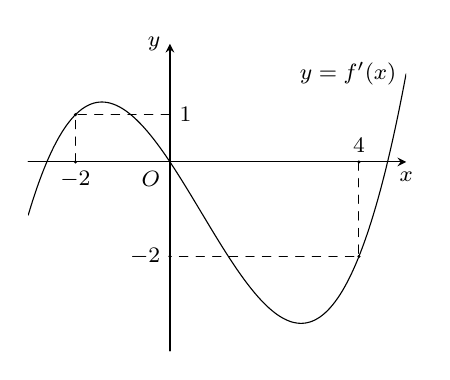
\begin{tikzpicture}[scale=0.6, font=\footnotesize, line join=round, line cap=round, >=stealth]
	\def\xt{-3} \def\xp{5} \def\yd{-4} \def\yt{2.5} 
	\draw[->](\xt,0) -- (0,0)node[below left]{$O$} -- (\xp,0)node[below]{$x$};
	\draw[->](0,\yd)--(0,\yt)node[left]{$y$};
	\begin{scope}
	\clip (\xt,\yd) rectangle (\xp,\yt);
	\draw[smooth,samples=150] plot[domain=\xt:\xp](\x,{0.125*(1*(\x)^3-2*(\x)^2-12*(\x))}) node[left]{$y=f'(x)$};
	\end{scope}		
	\draw[dashed](-2,0)--(-2,1)--(0,1) (4,0)--(4,-2)--(0,-2);	
	\foreach \i in {(4,0),(0,-2),(-2,0),(-2,1),(4,-2)} \fill \i circle(1pt);
	\path 
	(0,1) node[right]{$1$}
	(0,-2) node[left]{$-2$}
	(-2,0) node[below]{$-2$}
	(4,0) node[above]{$4$};
	\end{tikzpicture}
}
	\loigiai{\immini{Ta có $g'(x)=8xf'(x^2-4)+4x^3-16x$.\\
		Suy ra $g'(x)=0\Leftrightarrow g'(x)=0\Leftrightarrow\hoac{&x=0\\&f'(x^2-4)=-\dfrac{1}{2}\left(x^2-4\right).}$\\
			Xét $f'(x^2-4)=-\dfrac{1}{2}\left(x^2-4\right)$, đặt $t=x^2-4$ suy ra $f'(t)=-\dfrac{1}{2}t$.\\
			Trên hệ $Oxy$ với đồ thị hàm số $y=f'(x)$ vẽ đồ thị hàm số $y=-\dfrac{1}{2}x$ như hình vẽ bên.\\
			Khi đó $f'(x^2-4)=-\dfrac{1}{2}\left(x^2-4\right)\Leftrightarrow\hoac{&x^2-4=-2\\&x^2-4=0\\&x^2-4=4}\Leftrightarrow\hoac{&x=\pm\sqrt{2}\\&x=\pm 2\\&x=\pm\sqrt{8}.}$\\
			Bảng biến thiên của hàm số $y=g(x)$ như sau
				\begin{center}
				
\begin{tikzpicture}
				\tkzTabInit[espcl=1.5,lgt=1.5]
				{$x$/0.7,$y'$/0.7,$y$/1.8}
				{$-\infty$,$-\sqrt{8}$,$-2$,$-\sqrt{2}$,$0$,$\sqrt{2}$,$2$,$\sqrt{8}$,$+\infty$}
				\tkzTabLine{,-,0,+,0,-,0,+,0,-,0,+,0,-,0,+}
				\tkzTabVar{+/$+\infty$,-/$$,+/$$,-/$$,+/$$,-/$$,+/$$$$,-/$$,+/$+\infty$}
				\end{tikzpicture}
			\end{center}
			Vậy hàm số $g(x)$ có $4$ điểm cực tiểu.
		}
		{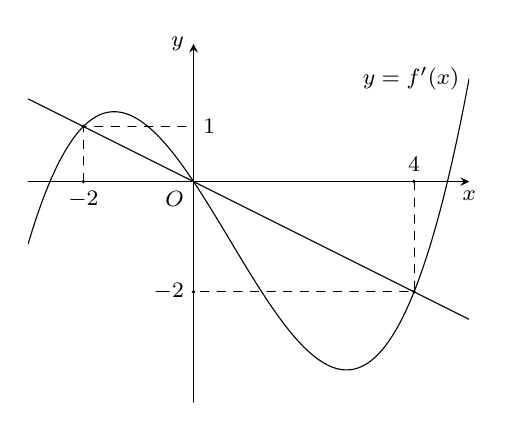
\begin{tikzpicture}[scale=0.7, font=\footnotesize, line join=round, line cap=round, >=stealth]
			\def\xt{-3} \def\xp{5} \def\yd{-4} \def\yt{2.5} 
			\draw[->](\xt,0) -- (0,0)node[below left]{$O$} -- (\xp,0)node[below]{$x$};
			\draw[->](0,\yd)--(0,\yt)node[left]{$y$};
			\begin{scope}
			\clip (\xt,\yd) rectangle (\xp,\yt);
			\draw[smooth,samples=150] plot[domain=\xt:\xp](\x,{0.125*(1*(\x)^3-2*(\x)^2-12*(\x))}) node[left]{$y=f'(x)$};
			\draw[smooth,samples=150] plot[domain=\xt:\xp](\x,{-0.5*(\x)});
			\end{scope}		
			\draw[dashed](-2,0)--(-2,1)--(0,1) (4,0)--(4,-2)--(0,-2);	
			\foreach \i in {(4,0),(0,-2),(-2,0),(-2,1),(4,-2)} \fill \i circle(1pt);
			\path 
			(0,1) node[right]{$1$}
			(0,-2) node[left]{$-2$}
			(-2,0) node[below]{$-2$}
			(4,0) node[above]{$4$};
			\end{tikzpicture}
		}
	}
\end{ex}
\begin{ex}%[Thi thử tốt nghiệp THPT- Cụm các trường THPT Nam Trực - Nam Định - 23]%[Phạm Tuấn B - EX6]%[2D3K2-4]
	Giả sử hàm số $y=f(x)$ liên tục, nhận giá trị dương trên $\left(0;+\infty\right)$ và thoả mãn $f(1)=1$, $f(x)=f'(x)\cdot\sqrt{3x+1}$, với mọi $x>0$. Mệnh đề nào sau đây đúng?
	\choice
	{\True $3<f(5)<4$}
	{$1<f(5)<2$}
	{$4<f(5)<5$}
	{$2<f(5)<3$}
	\loigiai{Do hàm số $y=f(x)$ liên tục, nhận giá trị dương trên $\left(0;+\infty\right)$ nên
		\allowdisplaybreaks
		\begin{eqnarray*}
		&&f(x)=f'(x)\cdot\sqrt{3x+1}\Leftrightarrow \dfrac{f'(x)}{f(x)}=\dfrac{1}{\sqrt{3x+1}}\\
		&\Rightarrow&\displaystyle\int\limits_1^5\dfrac{f'(x)}{f(x)}\mathrm{\,d}x=\displaystyle\int\limits_1^5\dfrac{1}{\sqrt{3x+1}}\mathrm{\,d}x\Leftrightarrow\ln\left|f(x)\right|\Big|_1^5=\dfrac{2}{3}\sqrt{3x+1}\Big|_1^5\\
		&\Leftrightarrow&\ln\left|f(5)\right|-\ln\left|f(1)\right|=\dfrac{2}{3}\left(4-2\right)=\dfrac{4}{3}\Rightarrow f(5)=\mathrm{e}^{\tfrac{4}{3}}.
		\end{eqnarray*}
	Vậy $3<f(5)<4$.	
	}
\end{ex}
\begin{ex}%[Thi thử tốt nghiệp THPT- Cụm các trường THPT Nam Trực - Nam Định - 23]%[Phạm Tuấn B - EX6]%[2D3K2-4]
	Cho hàm số $f(x)$ có đạo hàm trên khoảng $\left(0;+\infty\right)$ thoả mãn $f(x)=x\left[\sin x+f'(x)\right]+\cos x$ và $f\left(\dfrac{\pi}{2}\right)=\dfrac{\pi}{2}$. Giá trị của $f\left(\pi\right)$ bằng
	\choice
	{$1+\dfrac{\pi}{2}$}
	{$-1+\dfrac{\pi}{2}$}
	{$1+\pi$}
	{\True $-1+\pi$}
	\loigiai{Ta có với $x\in\left(0;+\infty\right)$ thì
		\allowdisplaybreaks
		\begin{eqnarray*}
		&&f(x)=x\left[\sin x+f'(x)\right]+\cos x\Leftrightarrow xf'(x)-f(x)=-x\cdot\sin x-\cos x\\
		&\Leftrightarrow& \dfrac{xf'(x)-f(x)}{x^2}=\dfrac{x(\cos x)'-\cos x}{x^2}\Leftrightarrow\left(\dfrac{f(x)}{x}\right)'=\left(\dfrac{\cos x}{x}\right)'\\
		&\Rightarrow&\displaystyle\int\limits_{\tfrac{\pi}{2}}^{\pi}\left(\dfrac{f(x)}{x}\right)'\mathrm{\,d}x=\displaystyle\int\limits_{\tfrac{\pi}{2}}^{\pi}\left(\dfrac{\cos x}{x}\right)'\mathrm{\,d}x\Leftrightarrow\left(\dfrac{f(x)}{x}\right)\Big|_{\tfrac{\pi}{2}}^{\pi}=\left(\dfrac{\cos x}{x}\right)\Big|_{\tfrac{\pi}{2}}^{\pi}\\
		&\Leftrightarrow&\dfrac{f(\pi)}{\pi}-\dfrac{f(\tfrac{\pi}{2})}{\tfrac{\pi}{2}}=-\dfrac{1}{\pi}\Rightarrow f(\pi)=\pi\left(1-\dfrac{1}{\pi}\right)=-1+\pi.
		\end{eqnarray*}
	}
\end{ex}
\begin{ex}%[Thi thử tốt nghiệp THPT- Cụm các trường THPT Nam Trực - Nam Định - 23]%[Phạm Tuấn B - EX6]%[2D3K2-4]
	Cho hàm số $y=f(x)$ liên tục trên đoạn $\left[0;1\right]$ và thoả mãn $\sqrt{x^3+1}\left[4xf'(1-x)-f(x)\right]=x^5$. Tích phân $I=\displaystyle\int\limits_0^1f(x)\mathrm{\,d}x$ có kết quả dạng $\dfrac{a-b\sqrt{2}}{c}$, ($a$, $b$, $c\in\mathbb{Z}^{+}$, $\dfrac{a}{c}$, $\dfrac{b}{c}$ là phân số tối giản). Giá trị $T=a-2b+3c$.
	\choice
	{$89$}
	{$27$}
	{$35$}
	{\True $81$}
	\loigiai{Thay $x=0$ vào $\sqrt{x^3+1}\left[4xf'(1-x)-f(x)\right]=x^5\Rightarrow f(0)=0$.\\
		Ta có
		\allowdisplaybreaks
		\begin{eqnarray*}
		&&\sqrt{x^3+1}\left[4xf'(1-x)-f(x)\right]=x^5\Leftrightarrow 4xf'(1-x)-f(x)=\dfrac{x^5}{\sqrt{x^3+1}}\\
		&\Rightarrow&\displaystyle\int\limits_0^14xf'(1-x)\mathrm{\,d}x-\displaystyle\int\limits_0^1f(x)\mathrm{\,d}x=\displaystyle\int\limits_0^1\dfrac{x^5}{\sqrt{x^3+1}}\mathrm{\,d}x.
		\end{eqnarray*} 
	Xét $\displaystyle\int\limits_0^1\dfrac{x^5}{\sqrt{x^3+1}}\mathrm{\,d}x$, đặt $\sqrt{x^3+1}=t\Leftrightarrow x^3+1=t^2$.\\
	Khi đó $x^2\mathrm{\,d}x=\dfrac{2}{3}t\mathrm{\,d}t$, đổi cận $\heva{&x=0\Rightarrow t=1\\&x=1\Rightarrow t=\sqrt{2}.}$\\
	Suy ra 	$\displaystyle\int\limits_0^1\dfrac{x^5}{\sqrt{x^3+1}}\mathrm{\,d}x=\displaystyle\int\limits_1^{\sqrt{2}}\dfrac{t^2-1}{t}\cdot\dfrac{2}{3}t\mathrm{\,d}t=\dfrac{2}{3}\left(\dfrac{1}{3}t^3-t\right)\Big|_1^{\sqrt{2}}=\dfrac{4-2\sqrt{2}}{9}$.\\
	Xét $\displaystyle\int\limits_0^14xf'(1-x)\mathrm{\,d}x$, đặt $1-x=t\Rightarrow\mathrm{\,d}x=-\mathrm{\,d}t$.\\
	Đổi cận $\heva{&x=0\Rightarrow t=1\\&x=1\Rightarrow t=0}$, khi đó
	\allowdisplaybreaks
	\begin{eqnarray*}
	&&\displaystyle\int\limits_0^14xf'(1-x)\mathrm{\,d}x=\displaystyle\int\limits_0^14(1-t)f'(t)\mathrm{\,d}t=\displaystyle\int\limits_0^14(1-t)\mathrm{\,d}(f(t))\\
	&=&4(1-t)f(t)\Big|_0^1+4\displaystyle\int\limits_0^1f(t)\mathrm{\,d}t=4\displaystyle\int\limits_0^1f(x)\mathrm{\,d}x.
	\end{eqnarray*}
	Suy ra $4\displaystyle\int\limits_0^1f(x)\mathrm{\,d}x-\displaystyle\int\limits_0^1f(x)\mathrm{\,d}x=\dfrac{4-2\sqrt{2}}{9}\Leftrightarrow\displaystyle\int\limits_0^1f(x)\mathrm{\,d}x=\dfrac{4-2\sqrt{2}}{27}$.\\
	Vậy $a=4$, $b=2$, $c=27$ nên $T=a-2b+3c=81$.
	}
\end{ex}
\begin{ex}%[Thi thử tốt nghiệp THPT- Cụm các trường THPT Nam Trực - Nam Định - 23]%[Phạm Tuấn B - EX6]%[2D2G6-5]
	Cho hàm số $f(x)=2^x-2^{-x}+2023x^3$. Biết rằng tồn tại số thực $m$ sao cho bất phương trình $$f\left(4^x-mx+37m\right)+f\left((x-m-37)2^x\right)\ge 0$$ có nghiệm đúng với $x\in\mathbb{R}$. Hỏi $m$ thuộc khoảng nào dưới đây?
	\choice
	{$\left(50;70\right)$}
	{$\left(-10;10\right)$}
	{\True $\left(30;50\right)$}
	{$\left(10;30\right)$}
	\loigiai{Ta có $f'(x)=\ln 2\left(2^x+2^{-x}\right)+2023\cdot 3x^2>0$ với mọi $x\in\mathbb{R}$ nên hàm số $f(x)$ đồng biến trên $\mathbb{R}$.\\
		Hơn nữa $f(-x)=2^{-x}-2^x-2023x^3=-f(x)$ nên $f(x)$ là hàm số lẻ.\\
		Khi đó,
		\allowdisplaybreaks
		\begin{eqnarray*}
		&&f\left(4^x-mx+37m\right)+f\left((x-m-37)2^x\right)\ge 0\\
		&\Leftrightarrow& f\left(4^x-mx+37m\right)\ge -f\left((x-m-37)2^x\right)=f\left((-x+m+37)2^x\right)\\
		&\Leftrightarrow& 4^x-mx+37m\ge (-x+m+37)2^x\Leftrightarrow 4^x+x\cdot 2^x-37\cdot 2^x- m\left(2^x+x-37\right)\ge 0\\
		&\Leftrightarrow&\left(2^x-m\right)\left(2^x+x+37\right)\ge 0\,(1).
			\end{eqnarray*}
	Xét hàm số $g(x)=2^x+x-37$ có $g'(x)=\ln 2\cdot 2^x+1>0$ với mọi $x\in\mathbb{R}$ nên hàm số $g(x)$ đồng biến trên $\mathbb{R}$.\\
	Mà $g(5)=0$ nên phương trình $g(x)=0$ có nghiệm duy nhất $x=5$.\\
	Vậy để bất phương trình ban đầu có nghiệm với mọi $x\in\mathbb{R}$ thì $2^x-m=0$ có nghiệm duy nhất $x=5$.	\\
	Suy ra $m=2^5=32$.
	}
\end{ex}
\begin{ex}%[Thi thử tốt nghiệp THPT- Cụm các trường THPT Nam Trực - Nam Định - 23]%[Phạm Tuấn B - EX6]%[2H1G3-6]
	Cho hình chóp $S.ABC$ có đáy là tam giác vuông cân tại $B$. Khoảng cách từ $A$ đến mặt phẳng $(SBC)$ bằng $a\sqrt{2}$, $\widehat{SAB}=\widehat{SCB}=90^\circ$. Khi độ dài cạnh $AB$ thay đổi, thể tích khối chóp $S.ABC$ có giá trị nhỏ nhất bằng
	\choice
	{$3\sqrt{3}a^3$}
	{$\dfrac{a^3\sqrt{2}}{2}$}
	{$a^3\sqrt{3}$}
	{\True $\dfrac{a^3\sqrt{6}}{2}$}
	\loigiai{\immini{Gọi $D$ là hình chiếu của $S$ trên $(ABCD)$.\\
			Do $\heva{&SD\perp CB\\&SC\perp CB}\Rightarrow DC\perp BC$	và $\heva{& SD\perp BA\\& SA\perp BA}\Rightarrow DA\perp BA$.\\
			Do đó $ABCD$ là hình vuông với cạnh $AB=x$.\\
			Do $AD\parallel BC\Rightarrow AD\parallel(SBC)\Rightarrow\mathrm{\,d}\left(A,(SBC)\right)=\mathrm{\,d}\left(D,(SBC)\right)$.\\
			Trong $\triangle SDC$ hạ $DH\perp SC\Rightarrow DH\perp(SBC)$.\\
			Suy ra $\mathrm{\,d}\left(A,(SBC)\right)=\mathrm{\,d}\left(D,(SBC)\right)=DH=a\sqrt{2}$.\\
			Mà $\dfrac{1}{SD^2}=\dfrac{1}{DH^2}-\dfrac{1}{DC^2}\Rightarrow SD=\dfrac{x\cdot a\sqrt{2}}{\sqrt{x^2-2a^2}}$.\\
			Suy ra $V_{S.ABC}=\dfrac{1}{3}\cdot SD\cdot S_{ABC}=\dfrac{1}{3}\cdot\dfrac{x^3\cdot a\sqrt{2}}{2\sqrt{x^2-2a^2}}$.\\
		}
		{\begin{tikzpicture}[scale=0.6, font=\footnotesize, line join=round, line cap=round, >=stealth]
			\tkzDefPoints{0/0/D}
			\coordinate (A) at ($(D)+(5,0)$);
			\tkzDefShiftPoint[D](-140:3){C}
			\coordinate (B) at ($(A)+(C)-(D)$);
			\coordinate (S) at ($(D)+(0,5)$);
			\coordinate (H) at ($(C)!0.5!(S)$);
			\tkzDrawSegments(S,C S,A A,B B,C S,B)
			\tkzDrawSegments[dashed](C,D D,H S,D A,D)
			\tkzDrawPoints[fill=black](A,B,D,C,H,S)
			\tkzLabelPoints[above](S)
			\tkzLabelPoints[below left](H)
			\tkzLabelPoints[right](A,B)
			\tkzLabelPoints[left](D,C)
			\end{tikzpicture}
		}
	\noindent
	Xét hàm số $f(x)=\dfrac{x^3}{\sqrt{x^2-2a^2}}$ với $x>a\sqrt{2}$.\\
	Ta có $f'(x)=\dfrac{2x^4-6a^2x^2}{\sqrt{\left(x^2-2a^2\right)^3}}\Rightarrow f'(x)=0\Leftrightarrow x=a\sqrt{3}$.\\
	Bảng biến thiên của hàm số $f(x)$ như sau
		\begin{center}
		
\begin{tikzpicture}
		\tkzTabInit[espcl=2,lgt=1.5]
		{$x$/0.7,$y'$/0.7,$y$/1.8}
		{$a\sqrt{2}$,$a\sqrt{3}$,$+\infty$}
		\tkzTabLine{,-,0,+}
		\tkzTabVar{+/$$$$,-/$3a^2\sqrt{3}$,+/$+\infty$}
		\end{tikzpicture}
	\end{center}
Suy ra $\min\limits_{\left(a\sqrt{2};+\infty\right)}f(x)=3a^2\sqrt{3}$.\\
Vậy thể tích khối chóp $S.ABC$ có giá trị nhỏ nhất bằng $\dfrac{a^3\sqrt{6}}{2}$.
	}
\end{ex}
\begin{ex}%[Thi thử tốt nghiệp THPT- Cụm các trường THPT Nam Trực - Nam Định - 23]%[Phạm Tuấn B - EX6]%[2D2G6-5]
	Có bao nhiêu cặp số $\left(x;y\right)$ với $x$, $y$ là các số nguyên thoả mãn đồng thời hai điều kiện sau \break $4\cdot 2^{y^4-2y^2}-2\log_2(2x)+x=0$ và $2\log_2\left(x+y\right)-x-y\ge 0$?
	\choice
	{$6$}
	{\True $2$}
	{$4$}
	{$9$}
	\loigiai{Xét hàm số $f(t)=2\log_2t-t$ với $t>0$.\\
		Ta có $f'(t)=\dfrac{2}{t\cdot \ln2}-1\Rightarrow f'(t)=0\Leftrightarrow t=\dfrac{2}{\ln 2}$.\\
		Hơn nữa $f(2)=f(4)=0$ nên bất phương trình $2\log_2t-t\ge 0$ có nghiệm $2\le t\le 4$.\\
		Khi đó $2\log_2\left(x+y\right)-x-y\ge 0\Leftrightarrow 2\le x+y\le 4$.\\
		Xét $4\cdot 2^{y^4-2y^2}-2\log_2(2x)+x=0\Leftrightarrow 2\cdot 2^{\left(y^2-1\right)^2}=2\log_2x-x+2$.\\
		Do $2^{\left(y^2-1\right)}\ge 1\Rightarrow 2\log_2x-x+2\ge 2\Leftrightarrow 2\le x\le 4$.
		\begin{itemize}
			\item Với $x=2$ thì $y^2-1=0\Leftrightarrow y=\pm 1$ nhưng $2\le x+y\le 4\Rightarrow y=1$.
			\item Với $x=3$ thì $2^{\left(y^2-1\right)^2}=3$, nên không tồn tại $y\in\mathbb{Z}$.
			\item Với $x=4$ thì $\left(y^2-1\right)^2=1\Leftrightarrow y=\pm 1$ do $2\le x+y\le 4$ nên $y=-1$.
		\end{itemize}
	Vậy có $2$ cặp số nguyên $\left(2;1\right)$ và $\left(4;-1\right)$ thoả mãn điều kiện bài toán.
	}
\end{ex}

\Closesolutionfile{ans}
\begin{indapan}{10}
	{ans/ans-2-TT-14-NamTruc-NamDinh-23}
\end{indapan}
